\documentclass{standalone}
\usepackage{tikz,trees}
\begin{document}
  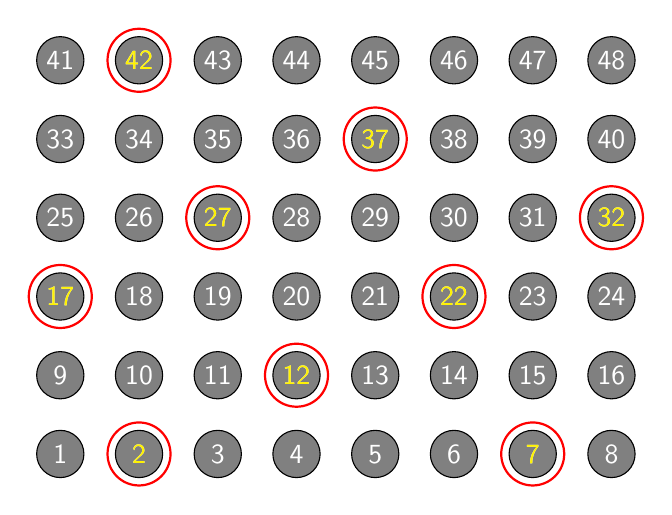
\begin{tikzpicture}[font=\sffamily]
    \foreach \num in {1,2,...,48} {
        \draw[fill=gray] ({\num - 8*floor((\num-1) / 8)},{floor((\num-1) / 8)}) circle (0.3) node[white] {\num};
    }
    \foreach \num in {2,7,...,42} {
        \draw[draw=red,thick] ({\num - 8*floor((\num-1) / 8)},{floor((\num-1) / 8)}) circle (0.4) node[yellow] {\num};
    }
  \end{tikzpicture}
\end{document}